\documentclass[11pt]{article}
\usepackage[margin=2cm,twoside]{geometry}
\usepackage{amsmath}
\usepackage{amstext}
\usepackage{units}
\usepackage{graphicx}
\title{Calculation of signals in the FMD simulation and reconstruction}
\author{Christian Holm Christensen}
\date{\today}
\def\MeV#1{\unit[#1]{MeV}}
\def\N#1{\unit[#1]{N}}
\def\Q#1{\unit[#1]{Q}}
\def\ALTRO{{\scshape altro}}
\def\RCU{{\scshape rcu}}
\def\FMD{{\scshape fmd}}
\def\VA{{\scshape va1}}
\def\class#1{{\small\ttfamily #1}}
\def\DeltaMip{\ensuremath{\bar{\Delta}_{mip}}}
\begin{document}
\maketitle 

\section*{Introduction}

This is meant as a reminder of what kind of manipulations we do in the
simulation and reconstruction of \FMD{} data.   Please refer to
\tablename~\ref{tab:conventions} for conventions and constants used in
this document. 

\begin{table}[Htbp]
  \begingroup
  \centering
  \begin{tabular}{|l|c|r|p{.6\textwidth}|}
    \hline
    \textbf{Symbol} & \textbf{Unit} & \textbf{Value} & \textbf{Description}\\
    \hline
    $\delta_{ij}$  & \MeV{}    &  & Energy loss by particle $j$ in strip $i$\\ 
    $\Delta_i$     & \MeV{}    &  & Summed energy loss in strip $i$\\
    ${}_{mc}$      &           &  & Monte-Carlo mark\\ 
    $q_{mip}$      & \Q{}       & 29.67 & Number of $e^-$ charges for a MIP\\
    $\DeltaMip{}$ & \MeV{}    & 0.124 & Average energy deposition by a MIP\\
    $c_i$          & \N{}      &  $[0,10^2-1]$ & ADC counts in strip $i$\\
    $g_i$          & \N{}/\Q{} & $~2.2$ & Pulser calibrated gain for strip $i$\\
    $p_i$          & \N{}      & $~100$ & Pedestal value in strip $i$\\
    $n_i$          & \N{}      & $2-4$ & Noise value of strip $i$\\
    $f_{ol}$       &           & 4 & On--line noise suppression factor\\
    $f_{reco}$     &            & 4 & Reconstruction noise suppression
    factor\\
    $b$           &           &  6 & Shaping time parameter\\
    $\rho$        & \unit[g\,cm\textsuperscript{-3}] & 2.33 & Density of silicon\\
    $T$           & \unit[cm] & 0.032 & Thickness of sensors\\
    \hline
  \end{tabular}
  \endgroup
  \vspace{1ex}
  \par
  \noindent Here, 
  \begin{align*}
    \DeltaMip{} &= \unit[1.664]{MeV cm^2 g^{-1}} \rho\,T\\
    &= \unit[1.664]{MeV cm^2 g^{-1}} \unit[2.33]{g\,cm^{-3}}
    \unit[0.032]{cm} \\
    &= \MeV{0.124}
  \end{align*}
  where $\rho=\unit[2.33]{g\,cm^{-3}}$ is the density of silicon, and
  $T=\unit[320]{\mu{}m}$ the thickness of the silicon sensor. 
  
  The factor $q_{mip}$ is given by the electronics of the front--end
  cards of the \FMD{} and was measured in the laboratory in August 2008.
  It is a digital--to--analogue setting corresponding to 1 MIP in the
  pulser injection circuit on the front--end electronics. 
  \caption{Conventions used in this document, and constant values.}
  \label{tab:conventions}
\end{table}


\section*{Simulations}

In the hits (\class{AliFMDHit}) are generated per strip for each
particle that impinges on a strip.  Stored in the hit are the energy
loss $\delta_{i,mc}$ of the particle impinging as well as the path
length $l_{i,mc}$ of the particle track through the strip.  

When generating simulated detector signal (\class{AliFMDSDigit} or
\class{AliFMDDigit}) the energy loss in all hits in a single strip is
summed to a total energy loss in the strip. 
\begin{equation}
  \label{eq:sim:sum_eloss}
  \Delta_{i,mc} = \sum_j \delta_{ij,mc} \quad[\MeV{}]
\end{equation}

The detector signal (ADC counts) is then calculated using the fixed
gain of the \VA{} pre-amplifiers ($q_{mip}$), the average
energy deposition of a MIP $\DeltaMip{}$, and the pulser calibrated
gain of the strip $g_i$.   These numbers combine to a conversion
factor $f_{i,mc}$ given by 

\begin{equation}
  \label{eq:sim:conversion_factor}
  f_{i,mc} = \frac{q_{mip} g_i}{\DeltaMip{}} \quad [\N{} \MeV{}^{-1}]
\end{equation}

This factor and the constant value $C_i$ is then used to calculate the
number of ADC counts 

\begin{equation}
  \label{eq:sim:adc_counts}
  c_i = \Delta_{i,mc} f_{i,mc} + C_i \quad[\N{}]
\end{equation}

In case of multiple samples ($r$) of the same strip, each sample $j$ is
given by
\begin{equation}
  \label{eq:sim:sub_adc_counts}
  c_{ij,mc} = f_{i,mc} \left(\Delta_{i,mc} + (\Delta_{i-1,mc}-\Delta_i) e^{-b
      \frac{j}{r}}\right)+C_i \quad[\N{}]
\end{equation}
where $j$ runs from 1 to $r$ (the number of samples), and $b$ is a
constant that depends on the shaping time of the \VA{}
pre-amplifier (see also \figurename~\ref{fig:sim:va1_response}). 

\begin{figure}[Htbp]
  \centering
  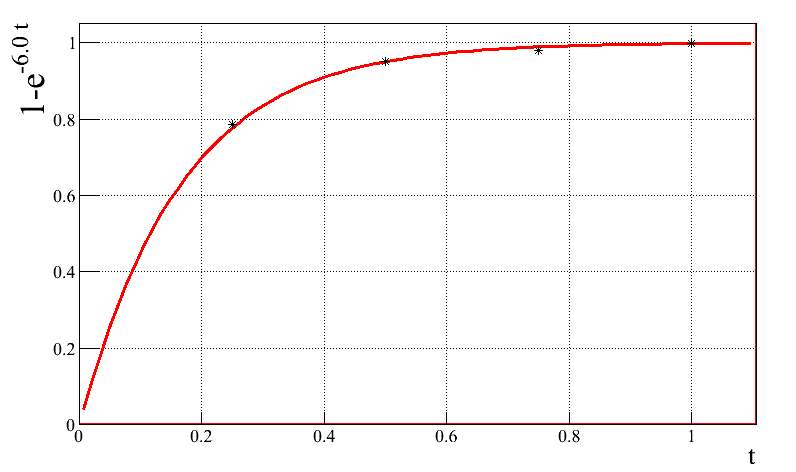
\includegraphics[keepaspectratio,width=.45\textwidth]{va1_response}
  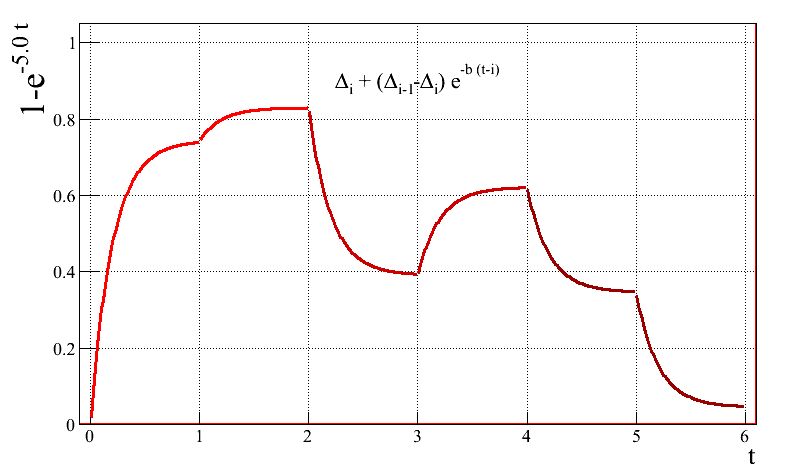
\includegraphics[keepaspectratio,width=.45\textwidth]{va1_train}
  \caption{Left: Shaping function of \VA{}, right: the resulting train
    of signals from \eqref{eq:sim:sub_adc_counts}. Note, that the
    signal value used is just before the turn to the next value.}
  \label{fig:sim:va1_response}
\end{figure}

Since the ADC has a limited range of 10bits ($=10^2-1=1024-1$) all
signals are truncated at 1023. 

For summable digits (\class{AliFMDSDigit}) $C_i=0$, but for 
fully simulated digits $c'_i$ (\class{AliFMDDigit}) it is given by
the pedestal $p_i$ and noise $n_i$ of the strip

\begin{equation}
  \label{eq:sim:pedestal_value}
  C_i = \text{gaus}(p_i,n_i)\quad[\N{}]
\end{equation}
that is, a Gaussian distributed number with $\mu=p_i$ (pedestal) and
$\sigma=n_i$ (noise). 

\section*{Raw data} 

The raw data, whether from simulation or the experiment, is stored in
the \ALTRO{}/\RCU{} data format.  The \ALTRO{} has 10 bit (maximum
count value of $\N{10^2-1}=\N{1023}$) ADC with up to 1024 consecutive
samples of the input signal.  The 128 input strip signals of \VA{}
chips, are multiplexed into a single \ALTRO{} channel in such a way
that each strip signal is sampled 1, 2, or 4 times\footnote{Currently,
  the default is to sample 2 times.}.  

The signal is then pedestal subtracted 
\begin{equation}
  \label{eq:sim:pedestal_subtraction}
  d_i = c_i - p_i + f_{ol} n_i\quad[\N{}]
\end{equation}
where $p_i$ and $n_i$ are the pedestal and noise value, evaluated
on--line in special calibration runs, and $f_{ol}$ is a integer factor
selected when configuring the detector\footnote{Typically $f_{ol}=4$.} 

After pedestal subtraction, which ensures that strips not hit by a
particle has a 0 signals, an zero--suppression filter is applied by
the \ALTRO{}.  This filter throws away all 0s from the data and
replaces them with markers that allows one to reconstruct the position
of the remaining signals in the sample sequence.  

The signals from each \ALTRO{} input channel is then packed into
blocks and shipped to the \RCU{} and eventually the data acquisition
system. 

In simulations a similar filter is applied to the data to simulate the
\ALTRO{} channels.  The total signal from the a strip
\eqref{eq:sim:adc_counts} is then given by 
\begin{equation}
  \label{eq:raw:sim_digits}
  c_i = \Delta_{i,mc} f_{i,mc} + \text{gaus}(p_i,n_i) - p_i - f_{ol} n_i \quad[\N{}]
\end{equation}
and similar for $c_{ij}$ \eqref{eq:sim:sub_adc_counts}.

\section*{Reconstruction} 

When reconstructing of either simulated data or data from the
experiment, the first thing is to read in the raw data stored in the
\ALTRO{}/\RCU{} data format\footnote{There is an option to reconstruct
  from the simulated \class{AliFMDDigit} objects directly, in which
  case this step is skipped entirely.}.  This is done by the
\class{AliFMDRawReader} class.  

Depending on whether or not the data was zero--suppressed, the
\class{AliFMDRawReader} code will do a pedestal subtraction, or add in
the noise previously subtracted in the \ALTRO{} (or simulation there
of) 

\begin{equation}
  \label{eq:reco:pedestal_subtraction}
  s'_i = c_i + C_i = c_i + \left\{
    \begin{array}{cl}
      - p_i & \text{not zero--suppressed}\\ 
      + f_{ol} n_i & \text{zero-suppressed} 
    \end{array}\right.\quad[\N{}]
\end{equation}
where $f_{ol}$ is the noise factor applied by the \ALTRO{}\footnote{This
  factor is stored in the event header and read by the
  \class{AliFMDRawReader} --- thus ensuring consistency.}, and $p_i$
and $n_i$ are the pedestal and noise value of the strip in question. 

In the reconstruction it is possible (via a \class{AliFMDRecoParam}
object) to specify a stronger noise suppression factor $f_{reco}$.  If
the signal $s'_i$ is smaller than the noise $n_i$ times the greater of
the two noise suppression factors, it is explicitly set to 0 
\begin{equation}
  \label{eq:reco:low_signal_cut}
  s_i = \left\{\begin{array}{cl}
    s'_i & s'_i > n_i \max{f_{ol},f_{reco}}\\
      0 & \text{otherwise}
    \end{array}\right.\quad[\N{}]
  \end{equation}

We now have a signal $s_i$ which is akin to $f_{i,mc}\Delta_{i,mc}$ of
\eqref{eq:raw:sim_digits}.  We therefor calculate the energy loss in
the $i^{\text{th}}$ strip using the factor 
\begin{equation}
  \label{eq:reco:conversion_factor}
  f_{i,reco} = \frac{\DeltaMip{}}{q_{mip} g_i} = f_{i,mc}^{-1}
  \quad[\N{}^{-1}\MeV{}]
\end{equation}
which is the inverse of \eqref{eq:sim:conversion_factor}, and the
energy loss is then  
\begin{equation}
  \label{eq:reco:energy_loss}
  \Delta_{i,reco} = s_i f_{i,reco}\quad[\MeV{}]
\end{equation}

\section*{From energy loss to ADC counts and back}

If we take \eqref{eq:sim:adc_counts} and \eqref{eq:reco:energy_loss}
and assume 
\begin{itemize}
\item that $s_i$ is not suppressed by \eqref{eq:reco:low_signal_cut}
\item \eqref{eq:reco:pedestal_subtraction} removes the fluctuations
  put in \eqref{eq:sim:pedestal_value}
\end{itemize}
and put them together we get 
\begin{align}
  \label{eq:all:all}
  \Delta_{i,reco} &= s_i f_{i,reco}\nonumber\\
  &= (c_i + C_i) \frac{\DeltaMip{}}{q_{mip} g_i}\nonumber\\
  &= \Delta_{i,mc} f_{i,mc}  f_{i,mc}^{-1}\nonumber\\
  &= \Delta_{i,mc}
\end{align}

\section*{Some calculations} 

Assuming a typical energy loss of \unit[2.9]{MeV\,cm\textsuperscript{-1}} and
applying \eqref{eq:sim:adc_counts} and
\eqref{eq:sim:conversion_factor}, we get a signal value over pedestal of
\begin{align}
  c_i &= \unit[2.9]{MeV\,cm^{-1}}\,T\, f_{i,mc}\nonumber\\
  &= \MeV{0.0928}\frac{\Q{29.67}\
    \unit[2.2]{N\,Q^{-1}}}{\MeV{0.124}}\nonumber\\
  &= \MeV{0.0928}\ \unit[526.40]{N MeV\textsuperscript{-1}}\nonumber\\
  &= \N{48.85}
\end{align}

\end{document}
